En esta sección haremos una breve introducción a algunas técnicas de Machine Learning y NLP que utilizamos a lo largo de esta tesis. Particularmente, ilustraremos y describiremos a grandes rasgos los últimos avances de Deep Learning para el área, desde \emph{word2vec} \cite{mikolov2013distributed} hasta la arquitectura Transformers \cite{vaswani2017attention}.

\section{Aprendizaje supervisado}

Muchas de las tareas de las áreas de Procesamiento de Lenguaje Natural, Visión por Computadora, Procesamiento del Habla (entre otras) pueden convertirse a problemas de aproximar una función $f: D \rightarrow O$, donde $D$ es el \emph{dominio} y $O$ el codominio o posibles salidas. Las funciones que es de nuestro interés aproximar son desconocidas, altamente no lineales y muy complejas. En el caso de que $O$ sea un conjunto finito, diremos que estamos ante un problema de \textbf{clasificación} y llamaremos a nuestro aproximador $\widehat{f}$ \textbf{clasificador} y a cada uno de las posibles salidas \textbf{clases}. En el caso de que $O$ conste de una o más variables continuas, decimos que estamos ante un caso de \textbf{regresión}. Para lo que concierne a esta tesis, nos centraremos en problemas de clasificación, así que restringiremos (salvo en los lugares donde se explicite lo contrario) nuestro análisis a este tipo de tareas.

Un ejemplo canónico de clasificación del área de Visión por Computadora es el de, dada una imagen de 28 x 28 píxeles en blanco y negro, predecir a cual de los 10 caracteres pertenece. En este caso, tenemos que $D$ es un subconjunto de ${0, 1}^{28 \times 28}$ --todas las imágenes posibles de ese tamaño en blanco y negro-- restringido a aquellas imágenes que correspondan a caracteres, y que $O = {0, 1, 2, \ldots, 8, 9}$ son las posibles salidas de esta función.

En el caso de NLP, uno de los que problemas que más veremos en esta tesis es el de clasificación de textos: dado un texto (un documento, un comentario en una red social) predecir alguna característica discreta de éste. Por ejemplo, si el texto es un comentario de una red social, podemos intentar identificar su polaridad: si es positivo, neutro, o negativo. O si el comentario en cuestión posee algún tipo de discriminación: en este caso tenemos como posibles salidas 0 (marcando no discriminatorio) o 1 en caso de que sí haya discriminación. Otro tipo de tarea es la de inferencia (Natural Language Inference o NLI): dadas dos oraciones de texto, predecir si una es una consecuencia lógica de la otra, si son independientes, o si son contradictorias. En este caso, el dominio son pares de oraciones de texto, y tenemos tres posibles salidas: contradicción, independiente, consecuencia.

Estos problemas que acabamos de describir son realmente difíciles de atacar mediante programas convencionales diseñados a través de heurísticas o reglas prefijadas \cite{bishop2006pattern}. En lugar de ello, los abordaremos mediante técnicas de \textbf{aprendizaje supervisado}, en el cual tendremos un conjunto de instancias $x_1, \ldots, x_n$ y sus respectivas etiquetas $y_1, \ldots , y_n$ que usaremos para entrenar nuestro aproximador $y \sim f^*(x)$. Este conjunto $\{ (x_1, y_1), \ldots (x_n, y_n)\}$ se denomina \textbf{conjunto de entrenamiento}.

El proceso de entrenamiento de un estimador consta de seleccionar una función $f\theta$ de un conjunto de candidatos $\{f_\theta: \theta \in \Sigma\}$, donde $\theta$ representa los parámetros del clasificador, y $\Sigma$ representa el conjunto de sus posibles valores. En el caso de un clasificador lineal (como una Support Vector Machine o una regresión logística) $\theta$ constará de un vector de $\mathbb{R}^n$. En el caso de redes neuronales (como las que veremos a continuación), constará de múltiples matrices y vectores correspondientes a sus diferentes capas.

\todo{Mencionar otras tareas que no estén mencionadas: transducción de secuencias, modelado de lenguaje}

Si bien en algunos capítulos de esta tesis utilizamos técnicas de clasificación lineal como Support Vector Machines y regresiones logísticas, nuestro eje está puesto en los modelos basados en redes neuronales. Estos modelos han logrado el estado del arte en NLP para casi cualquier tarea conocida, y pasamos a continuación a hacer un repaso de sus distintas variantes. Para una descripción de los modelos lineales, referimos a textos clásicos del área como \citet{bishop2006pattern}.

\section{Redes Neuronales}


Los \tbf{perceptrones multi-capa} (MLP) o \tbf{redes feed-forward} (FFN) son la ``quintaesencia'' de los métodos modernos de Deep Learning, como describen \citet{goodfellow2016deep}. Una de las primeros acercamientos a esta técnica es la neurona de McCulloch-Pitts \cite{mcculloch1943logical}, que intenta modelar parte del funcionamiento de las neuronas mediante una función:

\begin{equation*}
    y = H(\theta^T x)
\end{equation*}

\noindent donde $H$ es la función de Heaviside o función escalón, que vale $1$ si $x \geq 0$, y $0$ en otro caso. La neurona de McCulloch-Pitts permite aproximar a dos valores (0 ó 1), a partir de una entrada $x$ y un parámetro $\theta$. El perceptrón, desarrollado en 1958 en \citet{rosenblatt1958perceptron}, es el primer modelo que utiliza este tipo de modelo de cómputo cuyos parámetros se encuentran mediante un algoritmo. \citet{minsky1969perceptrons} demostraron que este tipo de modelos sólo pueden ajustarse a datos linealmente separables, provocando que por largo tiempo no se profundice en la investigación de redes neuronales.

Una forma de sortear estas dificultades planteadas es apilar (stack) estas neuronas para poder ajustar a más tipos de funciones. En términos matemáticos, esto es tan sólo una composición de funciones, tomando ahora $f = f_3 \circ f_2 \circ f_1$, donde $f_1$ es la primer ``capa'' de nuestra función correspondiente a la entrada, $f_2$ es la capa intermedia u oculta, y $f_3$ es la capa de salida, cada una teniendo sus parámetros $\theta_1, \theta_2, \theta_3$. Si bien este ejemplo consta de 3 capas, se puede generalizar a arbitrarias capas ocultas. Este modelo es el que conocemos como \textbf{Perceptrón Multicapa} o \textbf{Multi-Layer Perceptron} (MLP por sus siglas en inglés), y provocó el resurgir conexionista de las redes neuronales en los años 80s gracias al desarrollo de algoritmos que permitieron entrenar estos modelos mediante la técnica de backpropagation \cite{rumelhart1986learning}.

\citet{cybenko1989approximation} demostró que para cualquier función continua en el hipercubo de $\mathbb{R}^n$ existe una red neuronal con una función de activación sigmoidal de 3 capas que la puede aproximar infinitamente bien \footnote{La formulación del resultado es un poco más compleja pero escapa los fines de esta tesis}. Sucesivos resultados demostraron con mayor generalidad este resultado, para otras funciones de activación (como las ReLU) y otras arquitecturas. Dicho en términos coloquiales, este teorema asegura que para cualquier función podemos encontrar una MLP que la aproxima. Hay que notar, sin embargo, que estos teoremas aseguran existencia pero no son constructivos, y tampoco aseguran que el proceso de backpropagation nos lleve a esa solución \cite{goodfellow2016deep}. Tampoco nos dice qué tan grande tiene que ser la red neuronal para que pueda aproximar adecuadamente a la función objetivo. Teniendo estas salvedades en cuenta, estos teoremas (usualmente denominados como Teorema de Aproximación Universal de Redes Neuronales) aportan un sustento teórico de la potencialidad de estos algoritmos, refutando en cierto punto lo marcado por \citet{minsky1969perceptrons}.

\subsection{Redes neuronales recurrentes}

\begin{figure}
    \centering
    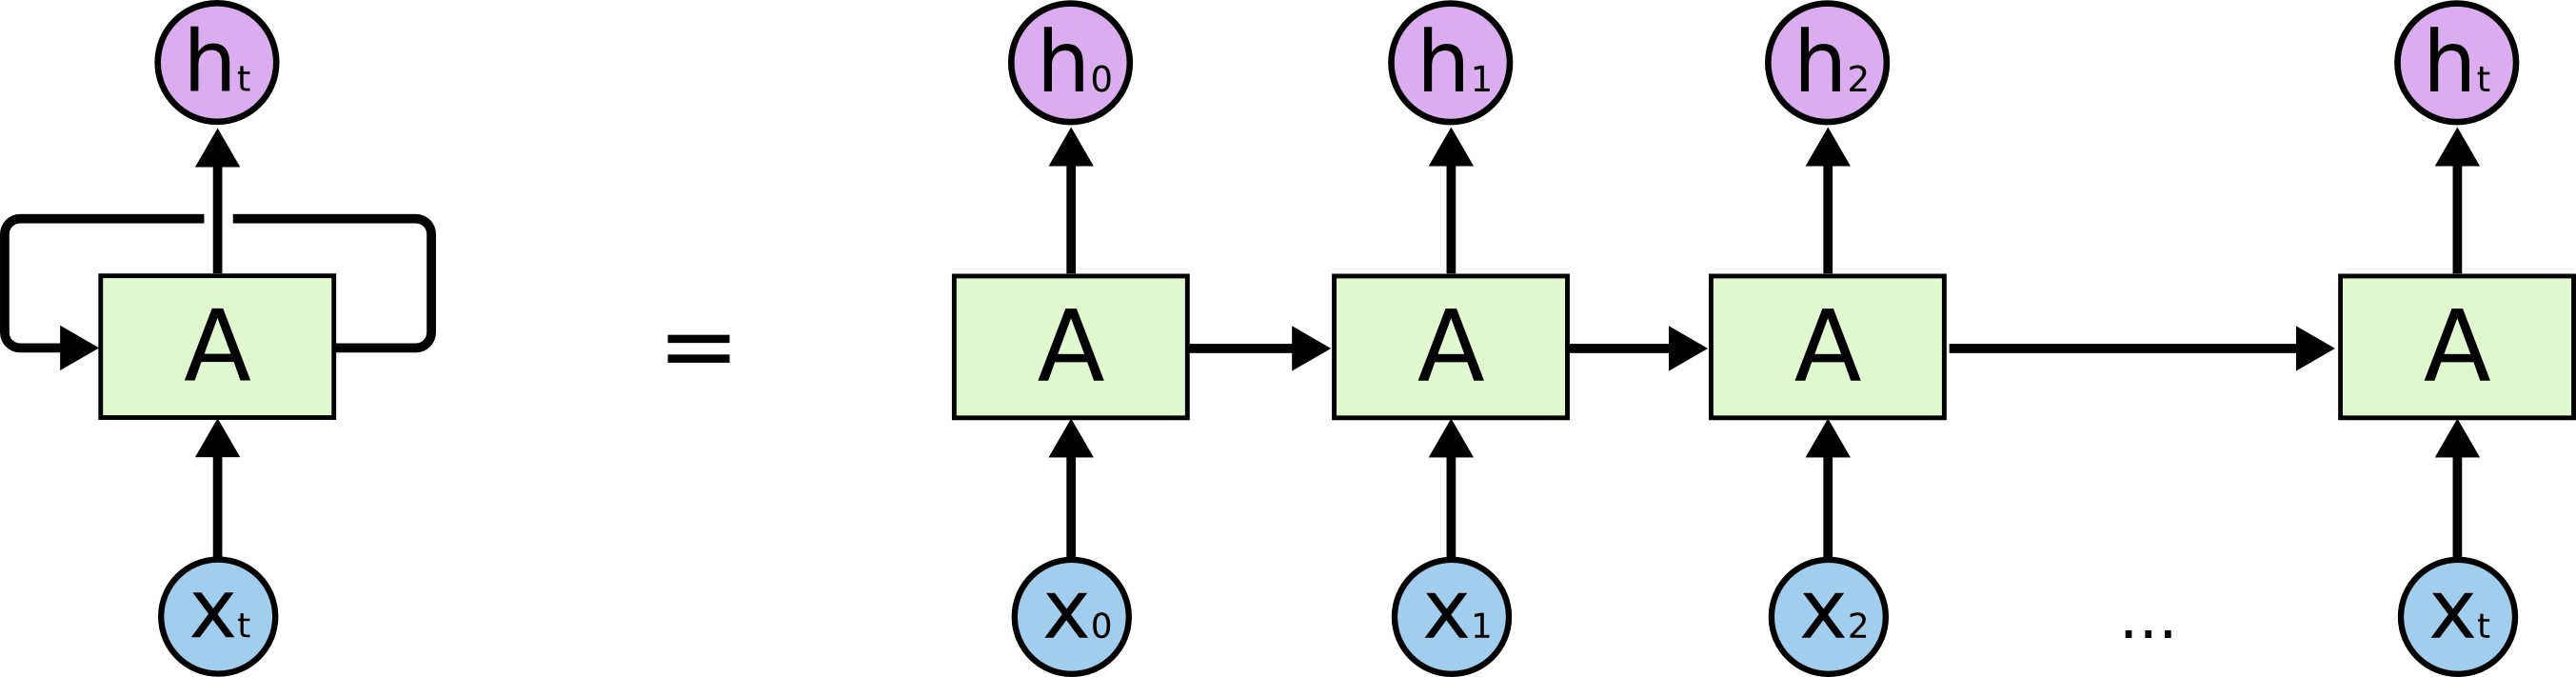
\includegraphics[width=0.8\textwidth]{img/rnn.png}
    \caption{Ilustración del esquema general de una red neuronal recurrente. Fuente: Blog de Christopher Olah}
    \label{fig:recurrent_net}
\end{figure}

Los problemas descriptos de NLP suelen constar de procesar una secuencia de palabras o tokens $x_1, x_2, \ldots, x_k$ de longitud variable, de manera de ajustar a una función

\begin{equation*}
    h = f([x_1, \ldots, x_k])
\end{equation*}

Una reformulación de este problema convirtiéndolo a una función que recibe una entrada de largo fijo es el de ajustar una función autorregresiva:

\begin{equation*}
    h_t = f(x_t, h_{t-1})
\end{equation*}

\noindent En este caso, tenemos una salida para cada paso $k$ de tiempo. Si $f$ es una red neuronal, llamamos a este tipo de redes neuronales \textbf{recurrentes}, ya que la salida a cada paso ($h_t$) depende de la salida del paso anterior, $h_{t-1}$. La figura \ref{fig:recurrent_net}  ilustra este esquema, tomada del excelente artículo de Chirstopher Olah sobre LSTMs \footnote{\url{https://colah.github.io/posts/2015-08-Understanding-LSTMs/}}. Una primer aproximación a las redes recurrentes es la red de Elman \cite{elman1990finding}, definida por las siguientes ecuaciones

\begin{align}
h_t &= \sigma(W_h x_t + U_h h_{t-1} + b_h) \\
y_t &= \sigma(W_y h_t + b_y)
\label{eq:elman}
\end{align}

\noindent donde $h_t$ es normalmente llamado el \textbf{estado oculto} en las redes neuronales recurrentes, e $y_t$ es la salida propiamente dicha. Los parámetros a ajustar son $W_h, U_h$ (matrices) y $b_h, b_y$ (escalares). Podemos ver que, a grandes rasgos, este tipo de red recurrente no es nada más que un perceptrón multicapa cuya entrada consta de $x_t$, la entrada original en el tiempo actual $t$, y el estado oculto anterior, $h_{t-1}$.

Para entrenar este tipo de redes recurrentes utilizamos back-propagation through time (BPTT), que consta en desplegar la relación recurrente --como está ilustrado en la figura \ref{fig:recurrent_net}-- y aplicar back-propagation de manera normal, poniendo un límite en la cantidad de pasos que tomamos hacia atrás. Las redes recurrentes de Elman sufren de varios problemas, principalmente de \textbf{vanishing gradient} y \textbf{exploding gradient}. Ambas dificultades pueden observarse ya que el cálculo del gradiente de las ecuaciones \ref{eq:elman} usando BPTT induce la potencia a la $n$ (donde $n$ es el largo de la secuencia) de las matrices $W_h$ y $U_h$, lo cual puede hacer o que bien el gradiente tienda a cero o a infinito. \footnote{ Esto puede verse usando alguna descomposición de la matriz como la forma normal de Jordan. Sus elementos en la diagonal que sean distintos de 1, o bien tienden a infinito o a cero.}

Los gradientes que tienden a infinito o \textbf{exploding gradient} pueden solucionarse mediante la técnica de \textbf{gradient clipping} \cite{goodfellow2016deep}, que consta de reajustar la norma del gradiente para que no exceda cierto valor. Sin embargo, nos queda aún el inconveniente de vanishing gradient. Para ello, se han propuesto otras arquitecturas recurrentes. \citet{hochreiter1997long} propusieron las \textbf{Long Short-Term Memory} (LSTM), una arquitectura basadas en compuertas (gates) que regulan el comportamiento del estado oculto y de la salida, evitando algunos de las dificultades de aprendizaje en las que incurre la red de Elman \footnote{Recomendamos el artículo antes mencionado de Christopher Olah para una muy buena explicación de este tipo de redes}. Otras arquitecturas como las Gated Recurrent Units \cite{cho-etal-2014-learning} usan menor cantidad de compuertas reduciendo la cantidad de parámetros a entrenar.

\section{Técnicas de representación}
\label{sec:02_representaciones}

Una de las necesidades que tienen las redes neuronales para poder trabajar con textos es el de tener representaciones continuas de cada token o palabra. Las representaciones utilizadas en la época previa de los donde reinaban los modelos lineales --bolsas de palabras/caracteres ponderadas con esquemas como TF/IDF-- adolecen de varios inconvenientes. En primer lugar, tienen una altísima dimensionalidad, usualmente del tamaño del vocabulario o algún límite similar. A su vez, no guardan representación semántica de la similaridad de las palabras: dos palabras como silla o banco tienen la misma distancia que perro y nube. Finalmente, sus valores no nulos están concentradas en una o pocas dimensiones y suelen ser discretas.

Latent Semantic Analysis (LSA) \cite{landauer1997solution} es una de las primeras técnicas de representación continua que tuvo cierta popularidad. Para obtener representaciones continuas de las palabras, plantean la factorización una matriz de co-ocurrencia entre tokens y documentos (o contextos) usando la descomposición SVD, obteniendo vectores de dimensión fija para los documentos y términos. LDA (Latent Dirichlet Allocation) \cite{blei2003latent} es otra técnica basada en modelos gráficos entrenados mediante métodos variacionales, muy utilizada aún en la actualidad ya que genera representaciones latentes de los tópicos de los textos.

%\begin{figure}
%    \centering
%    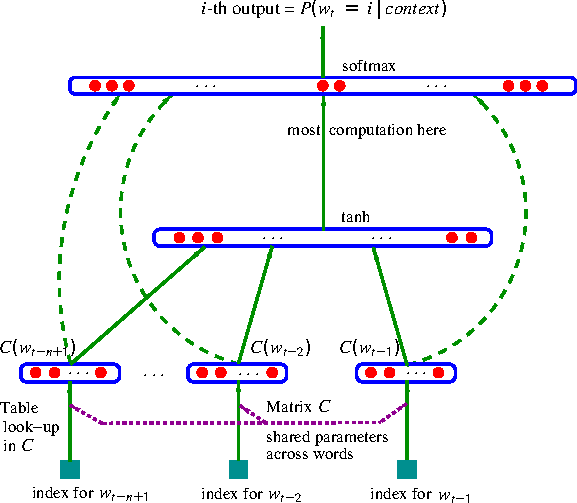
\includegraphics[width=0.65\textwidth]{img/02/bengio_neural_language_model.pdf}
%    \caption{Ilustración del modelo de lenguaje neuronal de \citet{bengio2003neural}. La entrada consta de $n-1$ palabras, que primero pasan por una lookup table (o capa de embeddings), una función de activación y son colapsadas para luego ser utilizadas como entrada de una función softmax.}
%    \label{fig:bengio_neural_language_model}
%
%\end{figure}

Dentro de los métodos neuronales, uno de los más populares ha sido el de \citet{bengio2003neural}, que propone una arquitectura neuronal para un modelo de lenguaje markoviano. %La arquitectura de esta red está ilustrada en la figura \ref{fig:bengio_neural_language_model}%.
En la capa intermedia contiene una tabla de lookup de vectores de las diferentes palabras (también conocido como capa de embeddings) donde se generan las representaciones de las palabras durante la etapa de entrenamiento. Trabajos posteriores (con diferentes variaciones de esta misma idea) como el de \citet{collobert2011natural} han demostrado que la utilización de este tipo de representaciones es útil para diversas tareas de NLP como POS Tagging, NER, y otras. Más aún, este trabajo tiene una idea que fue utilizada muchos años después con éxito rotundo: la utilización de la tarea de modelado de lenguaje como base para el pre-entrenamiendo de redes neuronales.

Uno de los problemas de los métodos comentados es que no son muy eficientes, sólo pudiéndose entrenar con pocos millones de palabras y con dimensiones reducidas. La técnica \emph{word2vec} \cite{mikolov2013efficient} permite entrenar representaciones de mayor dimensión y sobre grandes cantidades de textos de manera eficiente. Los vectores de palabras aprendidos guardan cierta estructura lineal y semántica, ilustrado por los autores con algunos ejemplos de analogías de palabras como el ya clásico $v(\text{rey}) - v(\text{hombre}) + v(\text{mujer}) \approx v(\text{reina})$.

Para generar los vectores de \emph{word2vec}, los autores plantean una relajación de la tarea de modelado de lenguaje mediante dos alternativas: Continuous Bag of Words (CBOW) y Skip-Gram. En CBOW se intenta predecir la palabra faltante dada una bolsa de palabras del contexto, mientras que Skip-gram se intenta predecir el contexto dada la palabra central, obteniendo en ambas variantes representaciones intermedias ricas. \citet{mikolov2013efficient} extiende la idea del anterior trabajo proponiendo plantear el problema de skip-gram como uno de distinguir palabras ruido de palabras efectivamente del contexto, haciendo mucho más eficiente el cálculo de estas representaciones. \emph{GloVe} \cite{pennington2014glove} es otra técnica de representación de palabras que combina las ideas de factorización de matrices de LSA  mediante un problema de optimización distinto y generando representaciones que superan ligeramente en algunos benchmarks de tareas a los de \emph{word2vec}.

Los métodos mencionados de representación calculan vectores de tamaño fijo sobre cada una de las distintas palabras. En español, por ejemplo, las palabras gato, gata, gatito, gatuno, todas tienen representaciones independientes en \emph{word2vec}, a pesar de tener información morfológica en común. Esto es un problema en varios escenarios: idiomas con muchas inflexiones o aglutinantes (como el turco, alemán o finés) o --lo que es de nuestro interés-- texto altamente desnormalizado como el de redes sociales. La técnica \fasttext{} \cite{bojanowski16} extiende la idea de \emph{word2vec} mediante la asignación de vectores a secuencias de 3 caracteres (subpalabras), capturando así cierta información morfológica. La representación de una palabra se obtiene mediante una combinación lineal de los vectores de las subpalabras que la componen.

\subsection{Embeddings a nivel oración}
\label{sec:02_tweet_embeddings}

%%
%%
%%
%%  https://docs.google.com/drawings/d/1BU3ulBiqU0NojpW6Fkb4xFlMCDigSWwfjN7z9smO6nY/edit
%%
%%

\begin{figure}[t]
    \centering
    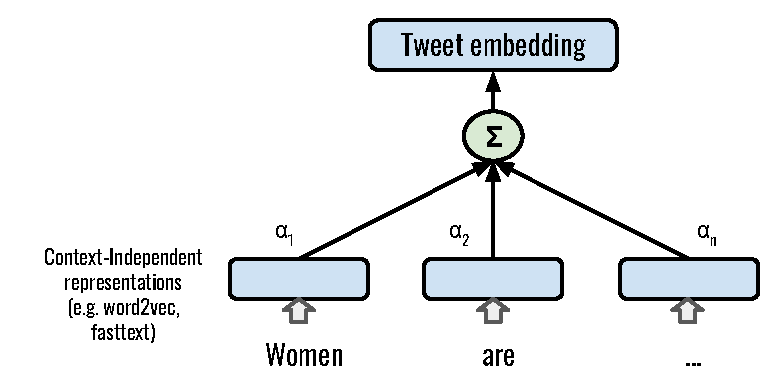
\includegraphics[width=0.75\textwidth]{img/tweet_embeddings.pdf}
    \caption{Representación continua de un tweet mediante combinación lineal de las representaciones de cada palabra.}
    \label{fig:tweet_embeddings}
\end{figure}

Una forma relativamente simple de obtener una representación de un texto \footnote{en nuestra tesis, esto será casi siempre un tweet} es realizar una combinación lineal de las representaciones obtenidas para cada palabra. Es decir, dada una oración $s = w_1 w_2 \ldots w_n$, y representaciones $\overline{w_1}, \overline{w_2}, \ldots, \overline{w_n} \in \mathbb{R}^m$, podemos obtener una representación

\begin{equation}
    \overline{s} = \sum\limits_{i=1}^{n} \alpha_i \overline{w_i}
\end{equation}

\noindent con $\alpha_1, \ldots, \alpha_n \in \mathbb{R}$ escalares (dependientes de la oración). De esta manera, obtenemos de $n$ representaciones independientes del contexto una representación para el tweet, sin tener en cuenta posibles interacciones entre los distintos componentes. La figura \ref{fig:tweet_embeddings} ilustra esta metodología simple para obtener representaciones de oraciones.

Tenemos entonces dos posibilidades para determinar la combinación lineal: la forma de obtener las representaciones, y la forma de calcular los coeficientes. Para las representaciones, podemos usar varias de las técnicas que ya vimos como \emph{word2vec}, \emph{GloVe}, o \fasttext{}. Para calcular los coeficientes, consideramos dos posibilidades. La primera, la forma canónica, calculando un promedio de las representaciones, es decir, tomando $\alpha_i = \frac{1}{n}$. Otra es realizar una ponderación usando Smooth Inverse Frequency (SIF) \cite{arora17}, inspirado en TF-IDF. Cada palabra $ w $ se pondera con $ \frac {a} {a + p (w)} $, donde $ p (w) $ es la probabilidad del unigrama  y $a$ es un hiperparámetro de suavizado. Los valores altos de $ a $ significan más suavizado hacia el promedio simple.



\section{Transfer Learning y modelos pre-entrenados}

\subsection{ELMo y ULMFiT}
\label{subsec:elmo}

Hasta cerca de 2018, la forma canónica de abordar un problema de NLP era entrenar una red neuronal recurrente que consumiera embeddings no contextualizados de los tokens de entrada. Esta arquitectura tiene algunas limitaciones; una de ellas es que, dados dos o más problemas distintos (por ejemplo, análisis de sentimientos y NLI) lo único compartido por ambas redes es la capa más baja --la capa de embeddings -- teniendo que entrenar desde cero todo el resto de los parámetros. En términos coloquiales, cada red debe ``aprender a leer'' sobre cada tarea, ignorando muchas construcciones sintácticas y semánticas comunes del lenguaje.

Uno de los esfuerzos exitosos en sobrepasar este abordaje es \elmo{} \cite{peters2018}. Este modelo aprende embeddings ya no sobre una única palabra como \emph{word2vec} sino sobre toda una oración, generando representaciones contextualizadas para cada una de ellas. \elmo{} se entrena sobre una tarea de modelo de lenguaje bidireccional \footnote{En realidad no es estrictamente bidireccional, sino dos LM concatenados} recurrente de varias capas sobre grandes cantidades de texto. En dicho trabajo, utilizan luego una combinación lineal de la salida de cada capa para obtener representaciones contextualizadas de cada token. Esta misma idea es una continuación de \citet{peters2017semi}, y también parcialmente de \emph{CoVe} \cite{mccann2017learned} donde construyen representaciones contextualizadas mediante la tarea de traducción automática.

\begin{figure}[t]
    \centering
    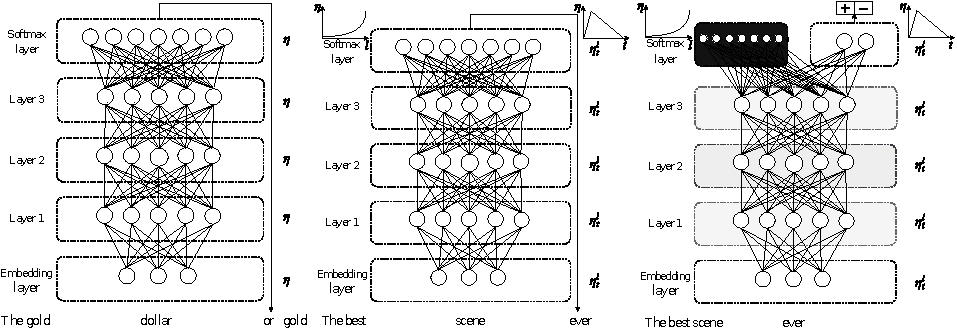
\includegraphics[width=\textwidth]{img/02/ulmfit.pdf}
    \caption{Universal Language Modeling for Text Classification (ULMFiT). Esquema del método planteado: primero se pre-entrena sobre la tarea de modelado de lenguaje sobre un dataset no supervisado. Luego, se corre la misma tarea pero sobre el texto de la tarea ignorando las etiquetas (ajuste de dominio). Finalmente, se agrega una capa de parámetros particulares de la tarea y se entrena la red completa descongelando gradualmente cada capa. Fuente: \citet{howard-ruder-2018-universal}}
    \label{fig:ulmfit}
\end{figure}

Alrededor de 2018, este paradigma de entrenar una red desde cero compartiendo su capa más baja --word2vec o bien \elmo{}-- comenzó a cambiar hacia un esquema donde se entrena una red neuronal sobre una tarea genérica para luego ajustarla a la tarea específica, una práctica muy común en el área de Visión por Computadora. \citet{howard-ruder-2018-universal} introdujeron la técnica de ULMFiT(Universal Language Modeling for Fine-tuning for text classification), uno de los trabajos fundamentales de este nuevo enfoque en NLP. ULMFiT consta de pre-entrenar en primer lugar un modelo de lenguaje sobre un gran dataset no etiquetado, y luego utilizar esa misma red (cambiándole la última capa) para ajustarla a una tarea específica. El primer paso, el \tbf{pre-entrenamiento} es realizado una única vez, y sus pesos son luego re-utilizados para realizar el ajuste en cada tarea distinta. Este es uno de los primeros esquemas de \tbf{transfer learning} exitosos sobre NLP: transferimos conocimiento de la tarea de modelado de lenguaje a las distintas tareas finales que realizamos como POS tagging, análisis de sentimientos, detección de entidades nombradas, etc.

Los autores proponen tres etapas: primero, el pre-entrenamiento sobre la tarea de modelado de lenguaje en un gran dataset de texto (e.g. Wikipedia o Common Crawl); segundo, un ajuste de la tarea de modelado de lenguaje sobre el texto de la tarea en cuestión (LM fine-tuning); y finalmente, el entrenamiento sobre las etiquetas de la tarea (Classifier fine-tuning). La figura \ref{fig:ulmfit} ilustra las tres etapas para el problema de clasificación de sentimientos. Entre varias técnicas que utilizan para entrenar estos modelos, vale destacar el uso de \emph{slanted triangular learning rates}, donde el learning rate tiene una etapa de \emph{warmup} donde sube hasta el pico y luego una etapa de \emph{annealing} donde se reduce linealmente hasta 0 por el resto del entrenamiento. Esta técnica es también utilizada por \bert{} y otros modelos de lenguaje basados en transformers.

El modelo de lenguaje utilizado por los autores de \emph{ULMFiT} utiliza una arquitectura \emph{AWD-LSTM} \cite{merity2018regularizing}. Estas arquitecturas recurrentes fueron el estado del arte para las tareas de modelado de lenguaje (y consecuentemente, para esquemas de transfer learning como el mencionado) pero fueron sobrepasados a los pocos meses por los modelos de lenguaje basados en \emph{transformers}.


\subsection{Traducción automática y atención}
\label{sec:02_transformers}


Hacemos a continuación una pequeña digresión sobre traducción automática y atención, conceptos necesarios antes de hablar de Transformers. El modelo \emph{encoder-decoder} permitió la utilización de redes neuronales para tareas de traducción de secuencias, es decir, donde queremos convertir $x = x_1 \ldots x_n$ a $y = y_1 \ldots y_m$, dos secuencias de diferente longitud. \citet{sutskever2014sequence} propusieron el siguiente esquema para abordar esta clase de tareas: en primer lugar, un \emph{codificador} (encoder) consume la cadena de entrada $x$,  conviertiéndola a un vector contextualizado $h$ de dimensión fija; y luego, un \emph{decodificador} (decoder) consume el vector de contexto $h$ para convertirlo a la cadena de salida $y$. Esto puede resumirse en las ecuaciones:

\begin{align*}
    h   &= \text{encoder}(x) \\
    y   &= \text{decoder}(h)
\end{align*}

Particularmente, los autores plantea un modelo basado en redes recurrentes (LSTMs) tanto para el \emph{encoder} como para el \emph{decoder}. El \emph{encoder} consume paso a paso la entrada, y el \emph{decoder} es esencialmente un modelo de lenguaje recurrente condicionado por el vector de entrada $h$.

Una de las limitaciones de las redes recurrentes es que sufren sesgo de \tbf{localidad} o \tbf{secuencialidad} (locality bias) \cite{battaglia2018relational}. En palabras coloquiales, las redes recurrentes tienen problemas para aprender dependencias de largo rango en las oraciones, siendo esto producto de su arquitectura autorregresiva donde se construye la salida $y_t$ en base a $y_{t-1}$. Este sesgo es particularmente dañino en tareas de tranducción de sequencias con la arquitectura encoder-decoder básica ya que a esto se le suma un cuello de botella forzoso por la compresión de toda la secuencia de entrada en el vector de dimensión fija $h$. Un síntoma de esto es observado en \citet{sutskever2014sequence}: invirtiendo la oración de entrada obtiene mejores resultados para la tarea de traducción automática.


\begin{figure}[t]
    \centering
    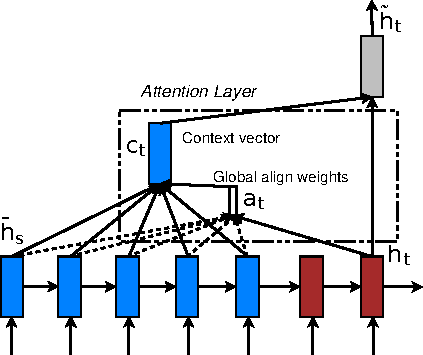
\includegraphics[width=0.5\textwidth]{img/02/attention_model.pdf}
    \caption{Mecanismo general de atención. En azul, la salida del encoder recurrente de la entrada. En rojo, la salida del decoder recurrente. Fuente: \citet{luong2015effective}}
    \label{fig:attention_mechanism}
\end{figure}


Los mecanismos de \emph{atención} \cite{bahdanau2014neural} ayudan a mitigar estas dificultades. A grandes rasgos, esta técnica agrega información adicional en cada paso del decoder mediante una combinación lineal de los estados ocultos del encoder. Recordemos que en la arquitectura básica propuesta en \citet{sutskever2014sequence} eran descartados, sólo siendo utilizado el estado final $h$. Describimos a continuación las ecuaciones de atención, que nos servirán para entender el mecanismo utilizado en la siguiente sección sobre Transformers.

Suponiendo que queremos traducir una secuencia $(x_1, \ldots , x_n)$ a $(y_1, \ldots , y_m)$, y que tenemos los estados ocultos $(\overline{h_1}, \ldots , \overline{h_n})$ generados en el encoder para la entrada, y los estados ocultos $(h_1, \ldots , h_m)$ y para la salida, el mecanismo de atención \footnote{global, en \citet{luong2015effective} se menciona el mecanismo local que no consideramos} consta de calcular para cada paso $t$ de la etapa de decodificación un vector de contexto

\begin{equation*}
    c_t = \sum_{i=1}^n \alpha_i^{(t)} \overline{h_i}
\end{equation*}

\noindent donde $\alpha^{(t)}$ es el vector de alineamiento, calculado como

\newcommand{\score}[0]{\text{score}}

\begin{equation*}
    \alpha^{(t)} = \softmax(\score(\overline{h_1}, h_t), \score(\overline{h_2}, h_t) \ldots , \score(\overline{h_n}, h_t))
\end{equation*}

\noindent Cada $\score(\overline{h_i}, h_t)$ marca una similaridad no normalizada entre sus argumentos. Las alternativas planteadas en \citet{luong2015effective} son:

\begin{equation}
    score(\overline{h_i}, h_t) =  \begin{cases}
        \overline{h_i}^T h_t   & \text{dot} \\
        \overline{h_i}^T W h_t & \text{general} \\
        v^T\text{tanh}(W [\overline{h_i}^T; h_t]) & concat
     \end{cases}
\end{equation}

% copypasting random stuff from the Internetz
% https://tex.stackexchange.com/questions/66537/making-hats-and-other-accents-bold
%
% \newcommand{\thicktilde}[1]{\mathbf{\tilde{\text{$#1$}}}}

\noindent con $W$ y $v$ parámetros adicionales. En el caso de la atención producto interno podemos reescribir todas las ecuaciones como:

\begin{equation}
    C = \softmax(H \widehat{H}^T ) \widehat{H}
    \label{eq:attention_product}
\end{equation}

\noindent donde $\widehat{H}, H$ son los vectores que tienen $(\overline{h_1}, \ldots , \overline{h_n})$  y $(h_1, \ldots , h_m)$ como filas respectivamente, y $\softmax$ se calcula fila a fila.

Finalmente, el vector $\widetilde{h_t}$ es calculado como una transformación del estado oculto del decoder $h_t$ y el vector contextual $c_t$:


\begin{equation*}
    \widetilde{h_t} = \tanh(W_h [h_t; c_t])
\end{equation*}


El vector $\widetilde{h_t}$ contiene información de todos los estados ocultos del codificador, atenuando los problemas de localidad de las redes recurrentes. Esta técnica se convirtió en parte integral de las tareas de traducción automática, resumen automático, entre otras. La figura \ref{fig:attention_mechanism} ilustra esta arquitectura.

La técnica de auto-atención o intra-atención \cite{parikh-etal-2016-decomposable} (self-attention en inglés) consiste en aproximadamente la misma idea que la atención sólo que teniendo una única secuencia; podemos asumir ecuaciones similares con $\overline{h_i} = h_i$. La auto-atención genera representaciones de los distintos vectores de entrada observando la totalidad de la secuencia, a diferencia de las redes recurrentes que sólo construyen una representación en base al paso anterior. Esta capa es utilizada en arquitecturas para clasificación de texto encima de una capa recurrente para generar representaciones con dependencias sin distinción de la distancia entre los distintos tokens.

\section{Transformers}

\begin{figure}[t]
    \centering
    \begin{subfigure}[t]{0.55\textwidth}
        \centering
        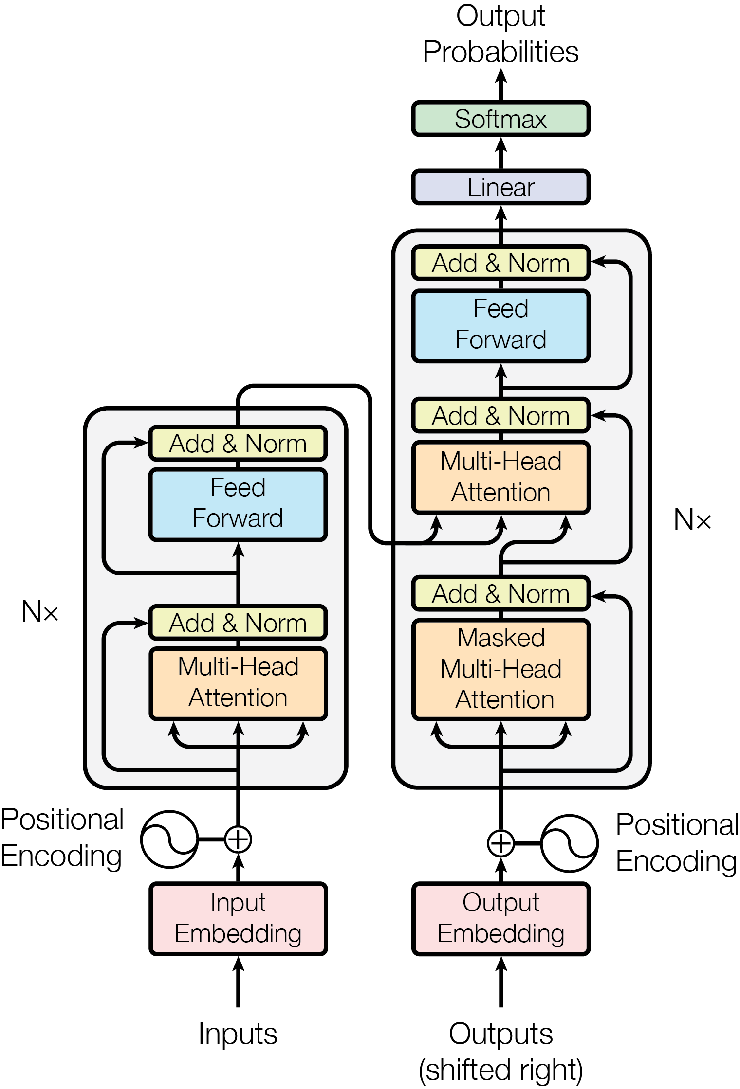
\includegraphics[width=0.55\textwidth]{img/02/transformer_architecture.png}
        \caption{Arquitectura de modelos Transformer}
        \label{fig:transformer_architecture}
    \end{subfigure}
    \begin{subfigure}[t]{0.40\textwidth}
        \centering
        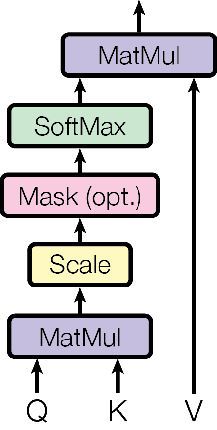
\includegraphics[width=0.40\textwidth]{img/02/scaled_self_attention.png}
        \caption{Mecanismo de scaled self-attention}
        \label{fig:scaled_self_attention}
    \end{subfigure}
    \caption{Modelo de transformador y su versión de auto-atención. La subfigura \ref{fig:transformer_architecture} muestra la arquitectura de los codificadores y decodificadores. Fuente: \citet{vaswani2017attention}}
    \label{fig:transformer_mechanism}
\end{figure}

Mencionamos el sesgo de la secuencialidad como uno de los problemas de las redes recurrentes. Otro de los grandes obstáculos para las arquitecturas autorregresivas es la paralelización. El cómputo secuencial donde $h_t$ se calcula en base a $h_{t-1}$ inhibe un cálculo paralelo, donde las diferentes representaciones puedan ser generadas simultáneamente. \citet{parikh-etal-2016-decomposable} es uno de los primeros trabajos que proponen una arquitectura para la tarea de inferencia (NLI) enteramente basada en una arquitectura de atención, sin ningún tipo de recurrencia.

\citet{vaswani2017attention} introdujeron la arquitectura \tbf{Transformer} para la tarea de traducción automática. Esta arquitectura no utiliza capas recurrentes ni convolucionales, basándose enteramente en el mecanismo de auto-atención. La figura \ref{fig:transformer_architecture} muestra la arquitectura de los modelos basados en Transformer, organizado en forma de encoder-decoder, con 6 capas de cada uno.

Cada capa del encoder utiliza un mecanismo de auto-atención múltiple seguido de una capa feed-forward punto a punto. Las dos capas de auto-atención o feed-forward están sucedidas por conexiones residuales \cite{he2016deep} para facilitar el flujo del gradiente en una arquitectura profunda y una capa de normalización, de manera que la salida se expresa como:

\begin{equation*}
    \text{Layer}(x) = \text{Norm}(x + \text{subLayer}(x))
\end{equation*}

Las capas decodificadoras son similares, salvo que se les agrega una capa extra de auto-atención donde se combinan las salidas del encoder con las representaciones que genera el decoder. A su vez, las capas de multi-atención están enmascaradas para no poder ``ver'' las representaciones que se generan en pasos posteriores para guardar su naturaleza secuencial en la tarea.

El cálculo de atención utilizado en este trabajo es similar al visto en la ecuación \ref{eq:attention_product}, aunque normalizado por $\sqrt{d_k}$, donde $d_k$ es la dimensión de los vectores de entrada:

\begin{equation*}
    Attention(Q, K, V) = \text{softmax}(\frac{Q^T K}{\sqrt{d_k}}) V
\end{equation*}

Cada capa utiliza varias cabezas de auto-atención, cuyas salidas son concatenadas y proyectadas. A su vez, la salida de cada una de las capa pasa por una regularización de tipo dropout \cite{srivastava2014dropout}.

Un punto a mencionar de los transformers es que, siendo que no tiene ningún tipo de recurrencia y convolución, carecen de cualquier ordenamiento de la secuencia de tokens. Para inyectar ese conocimiento en la red, utilizan \emph{vectores de posicionamiento} (positional embeddings) que se suman a los vectores de entrada de la capa de embeddings, como se ilustra en la figura \ref{fig:transformer_architecture}. Estos vectores no son parámetros entrenados (como sí lo son en \bert{}) sino que se calculan mediante funciones sinusoidales.


No nos extenderemos más en la explicación de esta arquitectura, y referimos para más información a los excelentes artículos \emph{Transformers from Scratch} \footnote{\url{http://peterbloem.nl/blog/transformers}}, \emph{Annotated Transformer} \footnote{\url{https://nlp.seas.harvard.edu/2018/04/03/attention.html}} y \emph{The Illustrated Transformer} \footnote{\url{https://jalammar.github.io/illustrated-transformer/}}.


\section{GPT, BERT y amigos}

\label{sec:02_bert}

Combinando las ideas de ULMFit --entrenamiento semi-supervisado sobre la tarea de modelado de lenguaje-- y la arquitectura Transformer --paralelización del cálculo mediante auto-atención -- en \citet{radford2018improving} se introduce GPT (\emph{generative pre-training}). Esta técnica consiste de un pre-entrenamiento sobre un gran corpus no etiquetado seguido de un fine-tuning discriminativo para cada tarea, muy en la línea de \citet{howard-ruder-2018-universal} introduciendo unos pocos parámetros específicos para cada una de estas. El modelo que usa esta tarea es el de \tbf{modelado de lenguaje causal} -- es decir, de izquierda a derecha. GPT obtuvo el estado de arte para el benchmark GLUE \cite{wang-etal-2018-glue}, superando a \elmo{} y otros.


\begin{figure}[t]
    \centering
    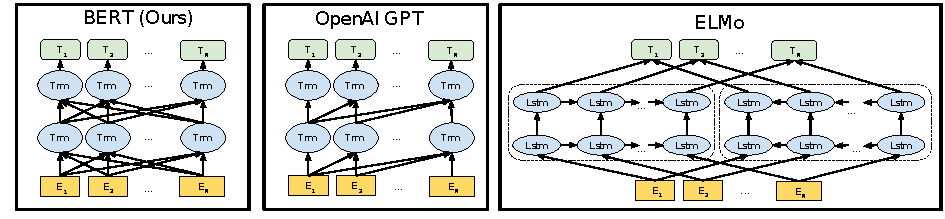
\includegraphics[width=\textwidth]{img/02/gpt_vs_bert.pdf}
    \caption{Comparación entre ELMo, GPT y BERT. ELMo genera vectores contextualizados mediante dos modelos de lenguaje recurrentes (uno de izquierda a derecha y el otro al revés), . GPT pre-entrena un modelo de lenguaje basado en Transformers. BERT genera representaciones bidireccionales }
    \label{fig:gpt_vs_bert_vs_elmo}
\end{figure}


\bert{} \cite{devlin2018bert} (Bidirectional Encoder Representations from Transformers) plantea una modificación sobre GPT: en lugar de pre-entrenar sobre la tarea de modelado de lenguaje \tbf{causal} --de izquierda a derecha-- hacerlo sobre la tarea de modelado de lenguaje \tbf{enmascarado}. Esta tarea (usualmente llamada \emph{Cloze task} \cite{taylor1953cloze}) consta de enmascarar una cierta cantidad de palabras de una frase, y luego intentar predecir las palabras faltantes. Por ejemplo, en la siguiente frase, consta de reemplazar los dos tokens \verb|[MASK]|:

\begin{center}
    El \verb|[MASK]| es celeste y el pasto \verb|[MASK]|
\end{center}


A diferencia de la tarea de modelado de lenguaje causal, los autores argumentan que esta tarea permite generar representaciones bidireccionales ricas. La figura \ref{fig:gpt_vs_bert_vs_elmo} muestra una comparación entre los distintos tipos de pre-entrenamiento de GPT.

BERT es pre-entrenado conjuntamente sobre dos tareas: una, la ya mencionada tarea de modelado de lenguaje enmascarado; la otra, la tarea de \emph{predicción de próxima oración} (Next Sentence Prediction, NSP). Esta tarea consiste en predecir si, dado un par de oraciones, la segunda es la que sigue a la primera. El 50\% de las ocasiones, las dos oraciones de entrada son contiguas en el texto de origen, y el 50\% restante son dos oraciones aleatorias concatenadas. Esta tarea debiera guardar cierta relación con la semántica de las oraciones y su interrelación, necesaria en tareas como NLI y Question Answering.

\newcommand{\clstok}[0]{\texttt{[CLS]}}
\newcommand{\septok}[0]{\texttt{[SEP]}}

\begin{figure}[t]
    \centering
    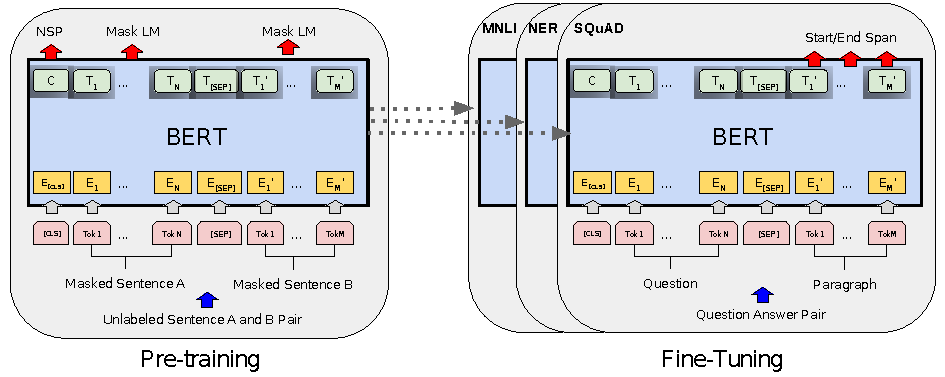
\includegraphics[width=\textwidth]{img/02/bert.pdf}
    \caption{Pre-entrenamiento y fine-tuning de BERT para distintas tareas. Fuente: \citet{devlin2018bert}}
    \label{fig:bert_pretraining_and_finetuning}
\end{figure}

Dos caracteres especiales son utilizados en \bert{}: \clstok{} y \septok{}. Estos caracteres se utilizan para delimitar las oraciones en la entrada de la red, y también para separar las dos oraciones de entrada. Durante el pre-entrenamiento, la representación generada por \clstok{} es utilizada como la predicción de la tarea NSP y la representación de cada token enmascarado es utilizado como entrada de una capa softmax para predecir el token faltante. Para la mayoría de las tareas de clasificación de texto, \clstok{} es usado como la representación de la (o las) oraciones de entrada. La figura \ref{fig:bert_pretraining_and_finetuning} ilustra esta metodología para la tarea de QA, ligeramente más compleja que la clasificación de texto.

\bert{} utiliza WordPiece \cite{wu2016google}, un algoritmo de tokenización muy similar a BPE \cite{sennrich2016neural}, con un vocabulario de largo 30,000 para separar su entrada en subpalabras de manera eficiente. A su vez, para cada posición de su entrada entrena embeddings posicionales (a diferencia de los embeddings posicionales fijos originales de \citet{vaswani2017attention}) con un límite de 512, y dos embeddings especiales para la primer oración y la segunda oración de la entrada. Los vectores que ingresan a la primer capa de transformers son la suma de los embeddings de cada token, los embeddings posicionales, y los embeddings de oración.

El proceso de pre-entrenamiento es realizado sobre la concatenación de dos corpus: BooksCorpus \cite{zhu2015bookscorpus} y la versión en inglés de Wikipedia. Estas dos fuentes son utilizadas ya que permiten extraer pares de palabras contiguas, algo necesario para la tarea de NSP.


\citet{liu2019roberta} proponen dos modificaciones al pre-entrenamiento de \bert{}: en primer lugar, remover la tarea de NSP; y en segundo lugar, realizar un pre-entrenamiento más extenso y con batch sizes más grandes, pasando de lotes de 512 a 8,192 oraciones. Este modelo pre-entrenado (al cual se denomina \roberta{}) obtuvo mejor desempeño que \bert{} en el dataset de GLUE y otras tareas.

Luego de estos modelos de lenguaje, una suerte de guerra armamentística tuvo lugar para entrenar arquitecturas más grandes y con más parámetros al observar que aumentando la cantidad de estos mejoraba la performance en distintas tareas -- sin observarse aún un techo más que los recursos computacionales y energéticos disponibles en el planeta. Sólo para ilustrar el punto, la versión \emph{base} de \bert{} tiene 110M parámetros, su versión large 330M, GPT-2 1,500M, Turing NLG de Microsoft 17,000M y finalmente GPT-3 \cite{brown2020language} tiene la asombrosa cantidad de 175,000 M parámetros.